\documentclass{article}

\usepackage[colorlinks]{hyperref}
\usepackage{booktabs}
\usepackage{graphicx}
\usepackage[svgnames]{xcolor}
\usepackage{minted}
\usepackage{fancyvrb}

\usepackage[many]{tcolorbox}

% https://tex.stackexchange.com/questions/181082/how-to-reproduce-this-box-in-tcolorbox
\newtcbox{\srcbox}{
  enhanced,
  nobeforeafter,
  tcbox raise base,
  boxrule=0.4pt,
  top=0mm,
  bottom=0mm,
  right=0mm,
  left=4mm,
  arc=1pt,
  boxsep=2pt,
  before upper={\vphantom{dlg}},
  colframe=teal!75!white,
  coltext=teal!25!black,
  colback=teal!5!white,
  overlay={
    \begin{tcbclipinterior}
      \fill[teal!75!white] (frame.south west) rectangle node[text=white,font=\sffamily\bfseries\tiny,rotate=90] {SRC} ([xshift=4mm]frame.north west);
    \end{tcbclipinterior}
  }
}

\newtcolorbox{featurebox}[1]{colback=teal!5!white,colframe=teal!75!white,title={#1}}

%%% Local Variables:
%%% mode: latex
%%% TeX-master: "capernaum-architecture"
%%% End:

\usepackage[export]{adjustbox}

% GitHub links
\newcommand{\ghtag}{arch-doc}
\newcommand{\ghurlprefix}{https://github.com/quantum-bits/capernaum/blob/\ghtag}
\newcommand{\ghurl}[1]{\ghurlprefix/#1}
\newcommand{\ghsrc}[4]{
  \begin{tcolorbox}[
    skin=enhanced,
    after title={\hfill\textsf{source link}},
    colframe=blue!50!white,
    colback=blue!5!white,
    hyperurl=\ghurl{#3}/\#L#4,
    title={#1}]
    #2
  \end{tcolorbox}
}

\newcommand{\screensnap}[1]{\includegraphics[width=\textwidth,cframe=blue!50!white 1pt]{images/#1}}

% Names for things
\newcommand{\caper}{\textsc{Capernaum}}
\newcommand{\boil}{\textsc{BoilerPlate}}
\newcommand{\cli}{\textsc{Cli}}
\newcommand{\gh}{\textsc{GitHub}}
\newcommand{\rest}{\textsc{Rest}ful}
\newcommand{\unix}{\textsc{Unix}}
\newcommand{\linux}{\textsc{Linux}}

% Named URLs
\newcommand{\ansible}{\href{https://www.ansible.com/}{\textsc{Ansible}}}
\newcommand{\apollo}{\href{https://www.apollographql.com/}{\textsc{Apollo}}}
\newcommand{\axios}{\href{https://axios-http.com/}{\textsc{Axios}}}
\newcommand{\bg}{\href{https://www.biblegateway.com/}{Bible Gateway}}
\newcommand{\bull}{\href{https://www.npmjs.com/package/bull}{\textsc{Bull}}}
\newcommand{\cfse}{\href{https://www.taylor.edu/center-for-scripture-engagement/}{\textsc{C4SE}}}
\newcommand{\cls}{\href{https://www.taylor.edu/center-for-scripture-engagement/survey/}{\textsc{Cls}}}
\newcommand{\dotenv}{\href{https://www.npmjs.com/package/dotenv}{\textsc{dotenv}}}
\newcommand{\filepond}{\href{https://pqina.nl/filepond/}{\textsc{FilePond}}}
\newcommand{\git}{\href{https://git-scm.com/}{\textsc{Git}}}
\newcommand{\gql}{\href{https://graphql.org/}{\textsc{GraphQL}}}
\newcommand{\grafana}{\href{https://grafana.com/grafana/}{\textsc{Grafana}}}
\newcommand{\handlebars}{\href{https://handlebarsjs.com/}{\textsc{Handlebars}}}
\newcommand{\jwt}{\href{https://jwt.io/}{\textsc{Jwt}}}
\newcommand{\nest}{\href{https://nestjs.com/}{\textsc{Nest}}}
\newcommand{\nginx}{\href{https://www.nginx.com/}{\textsc{nginx}}}
\newcommand{\nodemailer}{\href{https://nodemailer.com/}{\textsc{Node\-mailer}}}
\newcommand{\node}{\href{https://nodejs.org/}{\textsc{Node}}}
\newcommand{\pg}{\href{https://www.postgresql.org/}{\textsc{PostgreSQL}}}
\newcommand{\pmtwo}{\href{https://pm2.keymetrics.io/}{\textsc{Pm2}}}
\newcommand{\prometheus}{\href{https://prometheus.io/}{\textsc{Prometheus}}}
\newcommand{\qual}{\href{https://www.qualtrics.com/}{\textsc{Qualtrics}}}
\newcommand{\redis}{\href{https://redis.io/}{\textsc{Redis}}}
\newcommand{\tiptap}{\href{https://tiptap.dev/}{\textsc{TipTap}}}
\newcommand{\ts}{\href{https://www.typescriptlang.org/}{\textsc{TypeScript}}}
\newcommand{\tu}{\href{https://www.taylor.edu/}{TU}}
\newcommand{\typeorm}{\href{https://typeorm.io/}{\textsc{TypeOrm}}}
\newcommand{\vega}{\href{https://vega.github.io/vega-lite/}{\textsc{Vega-Lite}}}
\newcommand{\vuetify}{\href{https://vuetifyjs.com/}{\textsc{Vuetify}}}
\newcommand{\vue}{\href{https://vuejs.org/}{\textsc{Vue}}}
\newcommand{\websocket}{\href{https://developer.mozilla.org/en-US/docs/Web/API/WebSockets_API}{\textsc{WebSocket}}}

%%% Local Variables:
%%% mode: latex
%%% TeX-master: "capernaum-architecture"
%%% End:

% LocalWords:  Capernaum Cli ful Ansible Axios se Cls GraphQL Grafana Jwt
% LocalWords:  Qualtrics TypeORM Vuetify


\newcommand{\boilcmd}{\texttt{boil}}

\title{Streamlined Application Development\\with \boil}
\author{Dr.\ Tom Nurkkala}

\begin{document}
\maketitle
\tableofcontents

\section{Introduction}
\label{sec:introduction}

Many components of a database-backed web application
depend critically
on the specifics of the database schema.
For example:
\begin{enumerate}
\item Object-Relational Mapper (ORM) model classes
\item Data transfer objects (DTO's)
\item Database service classes
\item RESTful API resources
\item GraphQL object types, input types, and resolvers
\item UI CRUD views that maintain database content
\end{enumerate}
Creating
and updating
such components manually
can be tedious, inconsistent, and error prone.
Different components
rely on different aspects
of the underlying database schema
and may employ different naming conventions and
coding practices.

\boil{} consumes a JSON specification
for part of a database schema
(one entity and its relationships with other entities)
and generates ``starter code''
for one or more components whose
functionality depends on that portion of the schema.

\section{Usage}
\label{sec:usage}

Consider the snippet of a larger entity-relationship diagram (ERD)\footnote{View the
  \href{https://lucid.app/lucidchart/3b762a6b-a9f6-46fa-a54c-085f27f5b38d/edit?invitationId=inv_d358a7a6-5094-4a87-be16-4d7b25bad7ad}{full ERD}.}
shown in Figure~\ref{fig:erd}.
Our focus here is on the \texttt{Group} entity, which:
\begin{enumerate}
\item Stores attributes related a group respondents to an on-line survey
  (e.g., group name, information on the group administrator).
\item Has a many-to-one relationship with a \texttt{GroupType}
  (e.g., members of a civic group or university course).
\item Has a many-to-one relationship with a \texttt{Survey} entity
  (e.g., the survey to which group members will respond).
\end{enumerate}
Having defined this entity and its relationships,
our goal is to generate starter code that can 
access and manipulate \texttt{Group} data
in an underlying
relational database management system (RDBMS).

\begin{figure}
  \centering
  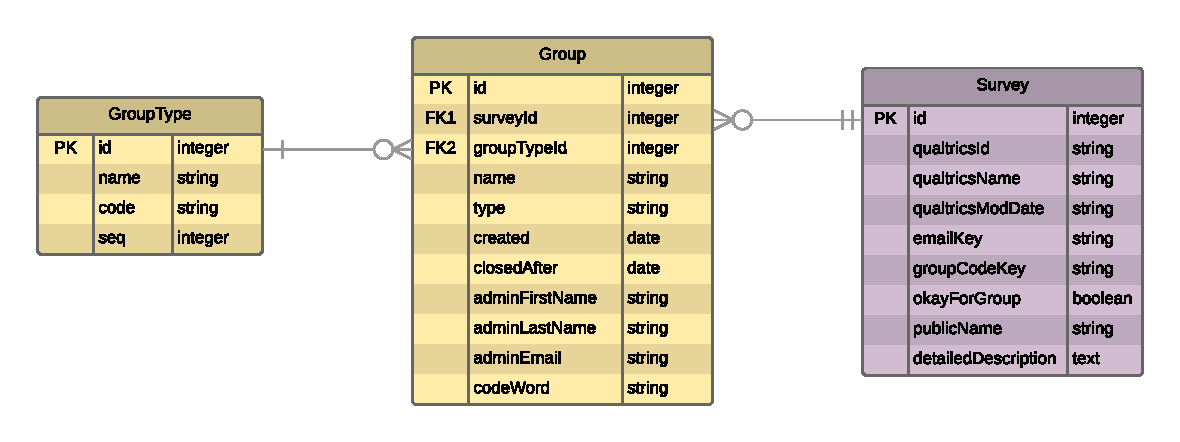
\includegraphics[width=\textwidth]{sample-erd}
  \caption{Entity-relationship diagram
    for the \texttt{Group}
    entity and related entities.}
  \label{fig:erd}
\end{figure}

\subsection{ERD Source File}
\label{sec:erd-source-file}

\boil{} is driven by a single JSON source file
that details a single \emph{entity},
its \emph{attributes}, and its \emph{relationships} with other entities.
Appendix~\ref{sec:erd-source}
shows the source file that corresponds to
the \texttt{Group} entity
from Figure~\ref{fig:erd}.

An ERD source file defines:
\begin{enumerate}
\item A single database entity, including its primary key and description.
\item Each attribute in the entity, including:
  \begin{enumerate}
  \item Type (e.g., \texttt{string}, \texttt{text},
    \texttt{float}, \texttt{date})
  \item Description
  \item Uniqueness
  \item Nullability
  \item Whether it should be exposed via \gql
\end{enumerate}
\item All relationships from the entity, including:
  \begin{enumerate}
  \item Name
  \item Description
  \item Destination entity
  \item Type (e.g., one-to-many, many-to-one, many-to-many)
  \item Nullability
  \end{enumerate}
\end{enumerate}

\subsection{Command}
\label{sec:command}


From an \hyperref[src:erd-source-file]{ERD source file}
the \boil{} command can generate various output files.
Figure~\ref{fig:help} shows the help output
from the main \boil{} command, \boilcmd,
which enumerates the types of output files it can generate.

Currently,
\boil{} is tailored to generate source files
that target
the \nest{} server-side framework
and a \vue-based web application using the \vuetify{} Material Design framework.
These targets are reflected in the following descriptions
of \boilcmd{} options.

\begin{figure}[hbt]
  \centering
\begin{Verbatim}[frame=single,framerule=1pt,rulecolor=blue!50!white]
Usage: boil [options] <schema-file>

generate boilerplate from an ERD file

Options:
  -e --entity         generate entity
  -m --module         generate module
  -r --resolver       generate resolver
  -s --service        generate service
  -t --table          generate Vue table
  -c --create-update  generate Vue create-update
  -a --all            generate all
  -b --banner         show banner before each section
  -v --verbose        be verbose
  -h, --help          display help for command
\end{Verbatim}
  \caption{\boil{} help output}
  \label{fig:help}
\end{figure}

\begin{description}
\item[\texttt{entity}]
  \ts{} class
  that includes decorators
  to define both a \typeorm{} database entity
  and a \gql{} object type,
  as well as \gql{} input types
  for inserting and updating the entity.
\item[\texttt{module}]
  \nest{} module file
\item[\texttt{resolve}]
  \gql{} resolver for CRUD operations
\item[\texttt{service}]
  \typeorm{} service for CRUD operations
\item[\texttt{table}]
  \vue{} component to display entity contents in a \vuetify{} table
\item[\texttt{create-update}]
  \vue{} component to create and update the entity
\end{description}

\subsection{Example Output}
\label{sec:output}

Table~\ref{tab:sample-output}
links to listings of \ts{} output
generated by \boil{}
when invoked with the indicated flag
on the ERD source file
shown in Appendix~\ref{sec:erd-source}.

\begin{table}[h]
  \centering
  \begin{tabular}{lll}
    \toprule
    Description                  & Flag                  & Listing                                                            \\
    \midrule
    \typeorm{} and \gql{} Entity & \texttt{-{}-entity}   & \hyperref[sec:output-entity]{Appendix~\ref{sec:output-entity}}     \\
    \typeorm{} Database Service  & \texttt{-{}-service}  & \hyperref[sec:output-service]{Appendix~\ref{sec:output-service}}   \\
    \gql{} Resolver              & \texttt{-{}-resolver} & \hyperref[sec:output-resolver]{Appendix~\ref{sec:output-resolver}} \\
    \bottomrule
  \end{tabular}
  \caption{Details of sample output from \boil}
  \label{tab:sample-output}
\end{table}


\section{Architecture}
\label{sec:architecture}

This section considers the architecture of \boil.
Refer to Figure~\ref{fig:block-diagram} for a block diagram.

\begin{figure}[h]
  \centering
  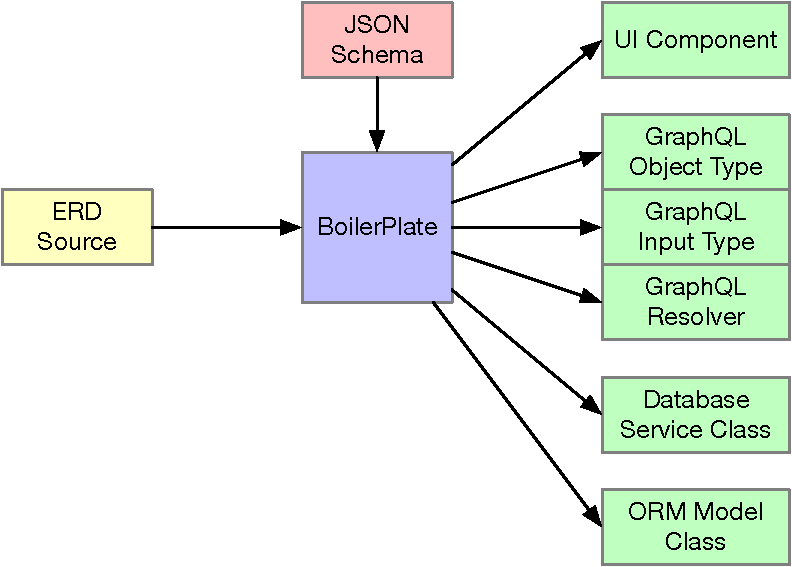
\includegraphics[width=0.8\textwidth]{block-diagram}
  \caption{
    \boil{} block diagram.
    The \textsf{ERD Source} input file
    must conform to the \textsf{JSON Schema}.
    Based on command-line flags,
    \boil{} generates one or more output files.
  }
  \label{fig:block-diagram}
\end{figure}

\subsection{JSON Schema}
\label{sec:json-schema}

\boil{} defines
a \href{https://json-schema.org/}{JSON Schema}
for the ERD source file,
allowing it to validate the file at run time.
In addition,
IDE's like
\webstorm{}
can read the JSON schema
and provide syntax checking and code hinting
while editing the ERD input file.

\ghsrc{JSON Schema}{
  JSON Schema describing the format of the ERD input file
  accepted by \boil.
}{schemata/er-schema.json}{1}

\subsection{Schema Classes}
\label{sec:schema-classes}

Corresponding to the contents of an ERD source file,
\boil{}
defines a family of classes
that represent the details the ERD,
including the entity, attributes, relationships,
and the schema itself.
\boil{} employs
the \href{https://www.npmjs.com/package/class-transformer}{\texttt{class-transformer}}
module to ``hydrate''
the ERD data from the source file
into these classes.
The classes themselves implement functionality
to process the details of the ERD.

\ghsrc{Schema Classes}{
  Classes, created from the ERD source file,
  that drive the generation of \boil{} output.
}{src/schema.ts}{1}

\subsection{Inflections}
\label{sec:inflections}

To keep names consistent across all output
generated by \boil,
it implements an ``inflection factory''
that converts root identifiers
into various forms
(e.g., initial capital, all caps, singular, plural, etc.).

\ghsrc{Inflection Factory}{
  The \texttt{Inflections} class
  generates various inflections
  of a root identifier
}{src/inflections.ts}{17}

\subsection{Templates}
\label{sec:templates}

\boil's \hyperref[sec:schema-classes]{schema classes}
process the ERD source data
into a form suitable for use in
\emph{templates} 
used to create the actual output files.
\boil{} uses \handlebars{}
for templating.

\ghsrc{Entity Template}{
  The entity in Appendix~\ref{sec:output-entity}
  was generated by instantiating this \handlebars{} template.
}{templates/graphql/entity.ts.hbs}{1}

\subsection{Extensibility}
\label{sec:extensibility}

As written, \boil{} is
tailored to generate code for 
\nest, \vue, and \vuetify.
However, its modular design
and use of standalone \handlebars{} templates
should allow it to be customized
to generate code
for other client- and server-side platforms.

\newpage
\appendix

\section{Listings}
\label{sec:listings}

This appendix contains listings cited previously.

\subsection{ERD Source}
\label{sec:erd-source}

Following is the JSON source for the \texttt{Group} entity (Figure~\ref{fig:erd}).
\inputminted[linenos,stepnumber=5,frame=single,fontsize=\small]{JSON}{sample-erd.json}

\subsection{Entity}
\label{sec:output-entity}

This is the \ts{} generated
by invoking \boil{}
with the \texttt{-{}-entity}
flag on the full ERD source file
for the \texttt{Group} entity
(Section~\ref{sec:erd-source}).

\inputminted[linenos,stepnumber=5,frame=single,fontsize=\small]{TypeScript}{group-entity.ts}

\subsection{Database Service}
\label{sec:output-service}

A \typeorm{} database service module
generated 
with \texttt{boil -{}-service}.

\inputminted[linenos,stepnumber=5,frame=single,fontsize=\small]{TypeScript}{group-service.ts}

\subsection{GraphQL Resolver}
\label{sec:output-resolver}

A \gql{} resolver module
generated 
with \texttt{boil -{}-resolver}.

\inputminted[linenos,stepnumber=5,frame=single,fontsize=\small]{TypeScript}{group-resolver.ts}

\end{document}

%%% Local Variables:
%%% mode: latex
%%% TeX-master: t
%%% End:

% LocalWords:  DTO's GraphQL GroupType Nullability
